%卒業論文概要テンプレート ver. 1.0

\documentclass[uplatex,twocolumn,dvipdfmx]{jsarticle}
\usepackage[top=22mm,bottom=22mm,left=20mm,right=20mm]{geometry}
\setlength{\columnsep}{15mm}
\usepackage[T1]{fontenc}
\usepackage{txfonts}
\usepackage{wrapfig}
\usepackage[expert,deluxe]{otf}
\usepackage[dvipdfmx,hiresbb]{graphicx}
\usepackage[dvipdfmx]{hyperref}
\usepackage{pxjahyper}
\usepackage{secdot}

\makeatletter
\renewcommand{\section}{%
  \@startsection{section}{1}{\z@}%
  {0.6\Cvs}{0.4\Cvs}%
  {\normalfont\normalsize\raggedright}}
\renewcommand{\subsection}{\@startsection{subsection}{2}{\z@}%
  {\z@}{\z@}%
  {\normalfont\normalsize}}
\renewcommand{\subsubsection}{\@startsection{subsubsection}{3}{\z@}%
  {\z@}{\z@}%
  {\normalfont\normalsize}}
\makeatother
%ここから上を編集する必要はない.





%タイトルと学生番号,名前だけ編集すること
\title{\vspace{-5mm}\fontsize{14pt}{0pt}\selectfont ビッグデータ処理技術を用いたWikipediaマイニング}
\author{\normalsize プロジェクトマネジメントコース・ソフトウェア開発管理グループ 矢吹研究室 1242005 石井康之}
\date{}
\pagestyle{empty}
\begin{document}
\fontsize{10.5pt}{\baselineskip}\selectfont
\maketitle





%以下が本文
\section{序論}

当研究では,Wikipedia の全編集履歴をデータマイニングすることによって,Wikipedia の管理者の動向を調査する.

ビッグデータとは,市販されているツールや従来のデータ処理で行うことが困難なほど巨大なデータ集合の集積物のことである.

Wikipediaとは,非営利のWikimedia財団がインターネット上で運営する,無料のオンライン百科事典プロジェクトである.このプロジェクトは匿名のボランティアの人々の協力によって日々動いている.Wikipediaの記事の品質が保たれて,現在も動いている理由として,管理者の存在が影響しているのではないかと考えた.

Wikipediaでは,プロジェクトが開始してから今までの全編集履歴データを提供している.このデータを扱うためにビッグデータ処理技術を用いることが出来る.

そこで当研究は,多言語版Wikipediaもデータ解析できる技術を得るために,ローカルで研究が行える環境を用意し,データマイニングを行う.


\section{目的}

Wikipediaを一つのプロジェクトとみなし,このオンライン百科事典で管理者の動向がどのように変化しているか調査する.

また,Wikipediaの編集履歴データを扱う際に必要なツールやプログラミングソースについての知識と,ビッグデータを扱う処理技術を得る.

\section{手法}

以下のとおり研究方法を行う.
\begin{enumerate}
 \item Wikipedia日本語版の編集履歴まで含んだファイルをダウンロードし,ローカルでデータマイニングを行う.
 \item Wikipediaの管理者の動向を解析する.
 \item 管理者の動向がプロジェクトの動きにつながっているのか調査する.
\end{enumerate}

\section{結果}

%図の挿入
%\begin{wrapfigure}[行数]{r}{幅}%行数はオプションだが,調整しないとうまくいかないことがある.
%\begin{wrapfigure}[11]{r}{4cm}
\begin{wrapfigure}{r}{4cm}
\vspace*{-\intextsep}
%\includegraphics[width=図の幅,clip]{ファイル名}\label{参照用ラベル}
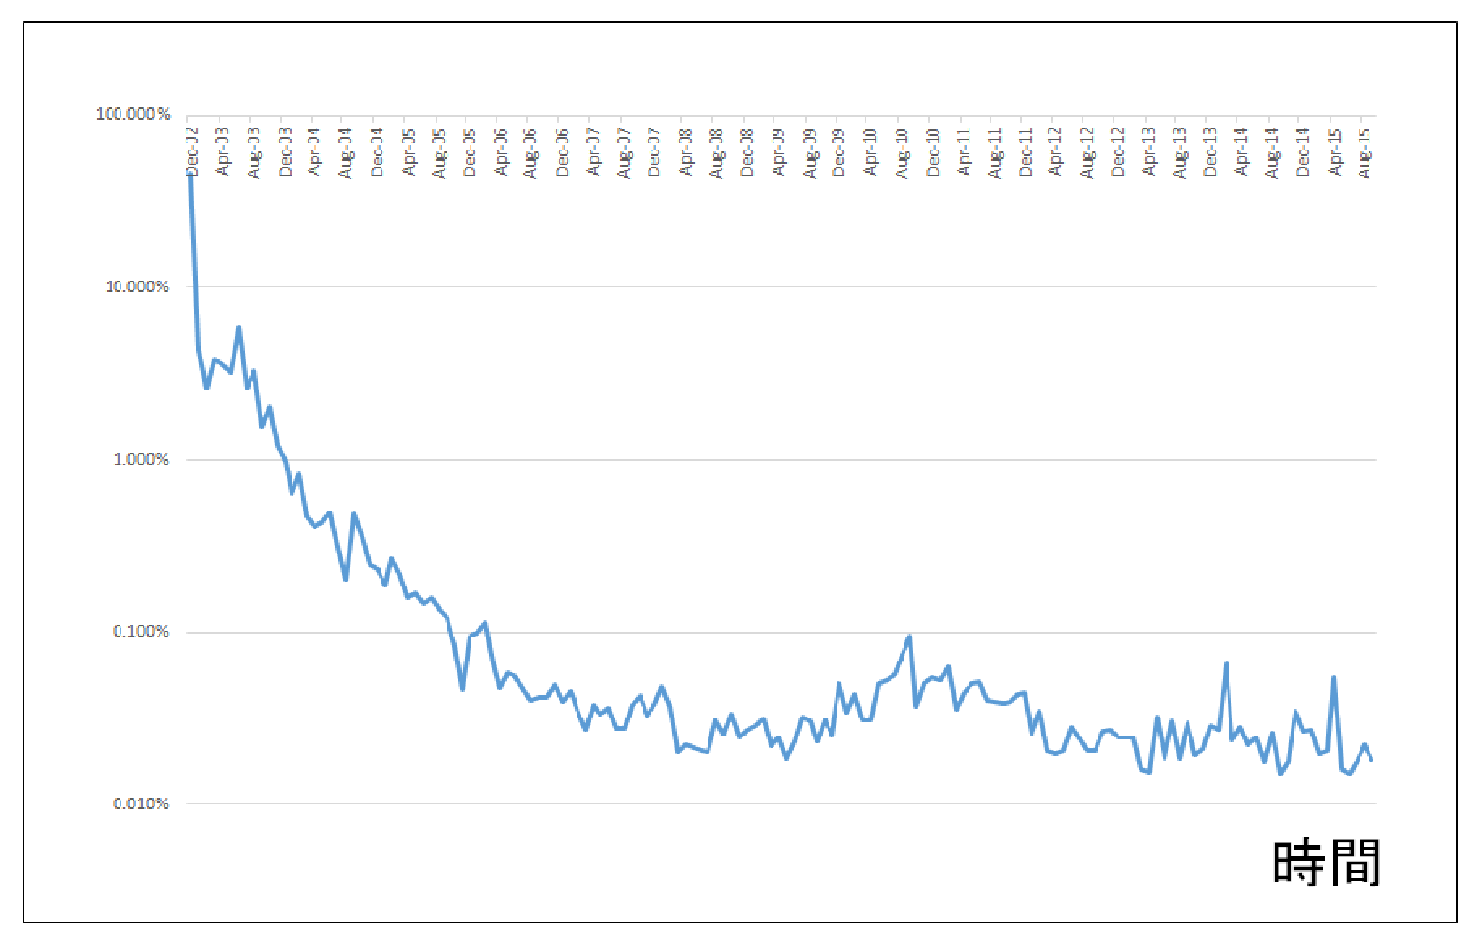
\includegraphics[width=4cm,clip]{editors_per.png}
\caption{管理者の月別動向の割合}\label{サンプル図}
\end{wrapfigure}

日本語版Wikipediaが実装されてからの,管理者の編集動向のデータ解析を行った.年々減少傾向になっている.


\section{考察}
日本のインターネット文化の「完全な匿名性」の普及が大きな要因と考えられる.\cite{wikirevo}
管理者になるとユーザー登録をすることになり,匿名での編集が出来ない.そのことが管理者の動向が減少していると考察する.

Wikipediaの編集履歴データを処理する際に,約10年分のデータを扱った.管理者の動向の調査だが「一般編集者から,途中から管理者になった編集者」の編集履歴の区別をすれば,更に正確なデータが取得できた.

\section{結論}

日本語版Wikipediaでは,管理者の動向が品質に影響しているわけではなかった.管理者が不足しているにもかかわらず,プロジェクトが日々動いている要因として,日本の文化はどこも比較的均一なため,あまり用法や言動についての論争があまり生まれないことが挙げられる.

管理者の動向を調査するため,約10年分のデータを扱い解析し,ビッグデータを扱う処理技術を得た.

\bibliographystyle{junsrt}
\bibliography{biblio}%「biblio.bib」というファイルが必要.

\end{document}